\chapter{Theory}

Before describing the work on friction estimation it is important to have some knowledge within vehicle dynamics, including basic knowledge on how tires and also different differentials work. The following chapter tries to describe this so that the reader has the right basic knowledge needed.

\section{Vehicle dynamics and models}

When looking at vehicle dynamics, there are many variables that are interesting to know. Some of these include the vehicles yaw rate, and the velocity and force generated in both lateral and longitudinal direction. The characteristics of a whole car is very complex and the behaviour of a car is therefore impossible to calculate in every situation. There exists many different car models that try to describe the characteristics of a car as adequate as possible. These calculations are also supposed to be done on a cars computer, which means that the model has to be simple enough to not reach the cars limited computing capacity.

\subsection{The bicycle model}

The bicycle model is a rather simple model that can be used to describe vehicle dynamics when turning, e.i. when we have a yaw rate and lateral forces that are affecting the vehicle. The models major simplifications are that the mass of the car is seen as one center of gravity point and that the two front wheels and the two rear wheels are combined into one wheel respectively as can be seen in Figure \ref{bicycle_model}. These simplifications mean that there is no difference in forces on the two sides, e.i. there will be no roll effect to the outside wheel when turning in a corner. There is also an assumption made that there will be no pitch effect on the car, which means that there is no suspension system that is effecting the car. The model also assumes that there is no driving torque generated to the wheels, and therefore only lateral forces on the vehicle.

For most cornering situations, these assumptions work fine, and the model gives a good idea on how different parameters are affected. Despite this, one has to bare in mind that these assumptions could result in rather large errors during certain driving situations.

\begin{figure}[h]
	\centering
	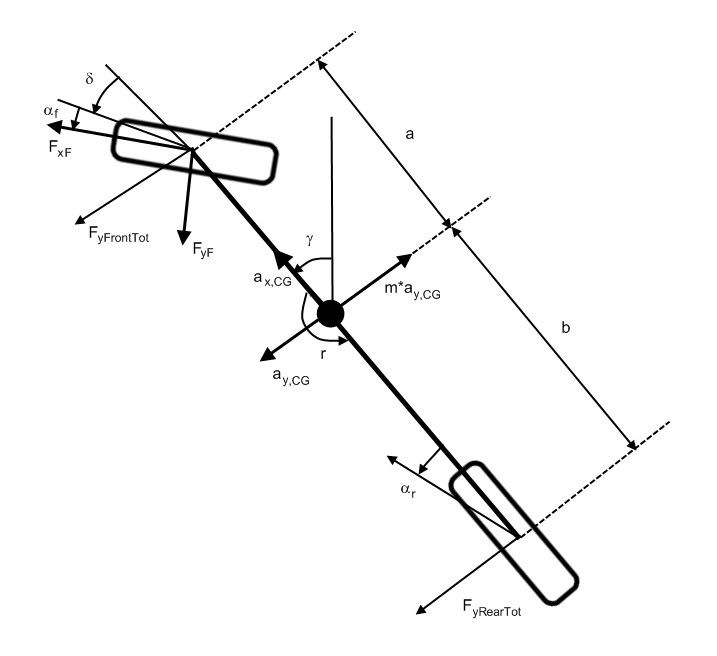
\includegraphics[width=0.8\textwidth]{Pictures/bicycle_model}
	\caption {Bicycle Model. \cite{fordonsdynamik99}}
	\label{bicycle_model}
\end{figure}

The total lateral force acting on the car will depend on the forces that the front and rear tires contribute with combined. By using Newtons second law of physics, $ F_{y} = m*a_{y} $, the total lateral force acting on the car will be
\begin{equation} \label{eq:lateral_force}
	F_{y} = m \cdot a_{y} = F_{yR} + cos(\delta) \cdot F_{yF} + sin(\delta) \cdot F_{xF} 
\end{equation}
where $ m $ denotes the vehicle mass, $ \delta $ is the front wheel steering angle. The acceleration in the center of gravity can be described as 
\begin{equation} \label{eq:lateral_acceleration}
	a_{y} = \dot v_{y} + \dfrac{F_{c}}{m}
\end{equation}
where $ \dot v_{y} $ is the actual change of velocity in lateral direction and the centripetal force in the center of gravity, $ F_{c} $, depends on the yaw rate
\begin{equation} \label{eq:yaw_rate}
	\dot \psi = \dfrac{v_{x}}{R}
\end{equation}
\begin{equation} \label{eq:centripetal_force}
	F_{c} = \dfrac{m \cdot v^2_{x}}{R} = mv_{x}*\dot \psi
\end{equation}
Where $ R $ is the radius of the turn and $ v_{x} $ the velocity in the direction that the car is pointing. By combining Equations \ref{eq:lateral_acceleration} and \ref{eq:centripetal_force}, the acceleration can described as
\begin{equation} \label{eq:lateral_acceleration_2}
	a_{y} = \dot v_{y} + v_{x}*\dot \psi
\end{equation}
When combining Equations \ref{eq:lateral_acceleration_2} and \ref{eq:lateral_force} the three different lateral force components that are effecting the vehicle can be described as
\begin{equation} \label{lateral_forces_2}
	F_{yR} + cos(\delta) \cdot F_{yF} + sin(\delta) \cdot F_{xF} = m*(\dot v_{y} + v_{x} \cdot \dot \psi)
\end{equation}
If taken one step further, the lateral force components can describe the torque created around the z-axis in the center of gravity 
\begin{equation} \label{yaw_bicycle}
	M_{z} = I_{z} \cdot \ddot \psi = a*(cos(\delta) \cdot F_{yF} + sin(\delta) \cdot F_{xF}) - b \cdot F_{yR}
\end{equation}
where $ a $ and $ b $ are the lever lengths from the center of gravity to the front respective the rear axle and $ \ddot \psi $ the yaw acceleration. 

When looking at the bicycle model,the assumption is that the longitudinal force is negligible. This means, as mentioned earlier, that the lateral force will almost only depend on the tire slip angle created by the front wheel steering angle and the angle to the direction the front wheel is heading towards. When assuming this model with only two wheels, the slip angles for the front respective rear tires will be
\begin{equation} \label{eq:wheel_slip_front}
	\alpha _{F} = -arctan(\dfrac{v_{y} + \dot \psi  \cdot a}{v_{x}}) + \delta
\end{equation}
\begin{equation} \label{eq:wheel_slip_rear}
\alpha _{R} = -arctan(\dfrac{v_{y} - \dot \psi  \cdot b}{v_{x}})
\end{equation}
This angle is defined to be the angle between the direction of the tire and the direction of the velocity of the wheel. A number of interpretations can be made from these formulas. One is that the steering angle only directly influences the slip angles of the front wheels. Another is that if the numerator in \ref{eq:wheel_slip_front} goes to zero, which means that the lateral velocity plus the yaw rate is zero, the slip angle of the front wheel is equal to the front wheel steering angle. This means that the vehicle is gliding straight forward regardless of the steering angle. Another conclusion is that if $ \dot \psi *b $ is larger than $ v_{y} $, in \ref{eq:wheel_slip_rear}, the numerator will become less then zero and slip angle of the rear wheel will move to the other side on the x-axis. This happens when a vehicle takes a corner more aggressively, which means higher longitudinal velocity compared to the radius of the corner, leading to higher yaw rate as can be seen earlier in \ref{eq:yaw_rate}.

The lateral forces acting on the front and rear wheels can also be described as 
\begin{equation}
	F_{yF} = 2C_{F}\alpha _{F}
\end{equation}
\begin{equation}
	F_{yR} = 2C_{R}\alpha _{R}
\end{equation}
where $ C_{F} $ and $ C_{R} $ are the lateral force coefficients for one front respective rear tire. The above calculations are taken from \cite{rajamani}. A steering response, $ B $, can de defined from these two forces \cite{fordonsdynamik99}
\begin{equation}
	B = F_{yR} - F_{yF}
\end{equation}
If $ B $ is 0, we have equal amount of lateral force on the front and rear wheels, which means that there is no under- or oversteer. Theoretically, this means that with a constant steering angle, the radius of the corner will be the same for all velocities. With a $ B < 0 $, a car has more force on the front tires, leading to that less and less steering angle is needed when the velocity increases in a corner. At one point, the steering angle will have to be negative to keep the radius of the corner. This phenomena is called understeer. If $ B > 0 $ on the other hand, more force will be on the rear tires and more steering angle is needed to keep the radius of a corner when increasing the velocity. This kind of behavior is called understeer. A slight understeer is usually desired for commercially available cars because handling of the car becomes easier and the risk of skidding is reduced.

\subsection{Two track vehicle model}

The bicycle model described earlier is a simplified car model that only captures the main characteristics well in many situations. The fact that it is modeled by only one wheel per axis means that the forces on the two wheels on the same axis will be modeled exactly the same. In reality, there will of course exist factors that affect the two wheels different, e.g. when cornering, the normal force will be transfered from the inner to the outer wheel. If a car uses an FXD, the active differential will in certain situations transfer torque from one shaft to the other. The effect that the FXD contributes with will be described further on in a later section of the paper. A model that is slightly more complicated than the bicycle model,  that tries to capture these lateral differences, is the two track model seen in \ref{two_track_model}. 

\begin{figure}[h]
	\centering
	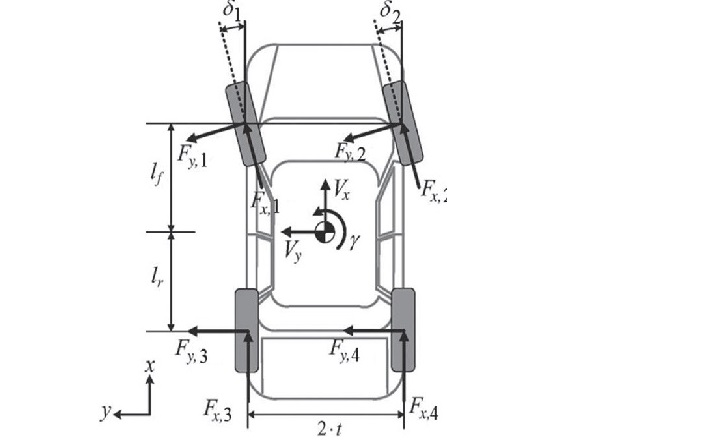
\includegraphics[width=0.8\textwidth]{Pictures/two_track_model}
	\caption{Forces acting on the car with a two track model.}
	\label{two_track_model}
\end{figure}

A couple of assumptions are made in this report when considering the two track model. There will never be a steering angle on the rear wheels and also the steering angle of the two front wheels are considered to be identical. Cars that are using an FXD are exclusively front wheel driven, and therefore the rear wheels will never contribute with positive forces. 



\subsection{Normal forces}

The longitudinal and lateral forces that act on the tires are dependent on the normal forces. It is therefore interesting to know how much normal force that's acting on each tire in order to find out how much longitudinal and/or lateral force the tires can transfer.

\subsubsection{Lateral influence}

\begin{figure}[h]
	\centering
	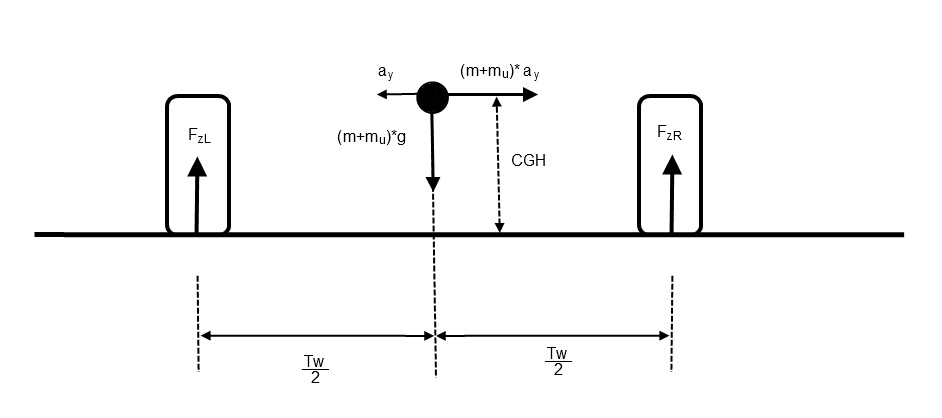
\includegraphics[width=0.8\textwidth]{Pictures/normal_force_lateral}
	\caption{Normal force on the car seen from the front.}
	\label{normal_force_lateral}
\end{figure}
Without any lateral acceleration, the normal forces on the right and left hand side of the car, as seen in Figure  \ref{normal_force_lateral}, can simply be described as
\begin{equation} \label{eq:normal}
	F_{zL} + F_{zR} = mg
\end{equation}
With lateral acceleration affecting the car, a torque will occur that changes the normal forces on the two sides. 
\begin{equation} \label{eq:normal_with_lat_acc}
	F_{zR}*T_{w} = mg*\frac{T_{w}}{2} + m*a_{y}*CGH
\end{equation}
where $ T_{w} $ is the track width, or distance between the wheels, $ a_{z} $ the lateral acceleration and $ CGH $ the height from the ground to the center of gravity. The torque that is an effect of the lateral acceleration in Equation \ref{eq:normal_with_lat_acc}, does not take account for that the center of gravity height will change during driving.

When taking a corner, there will also be load transfer from the inner to the outer wheel, which will depend on the centripetal force, $ F_{c} = ma_{y} $, and the load transfer coefficient $ \sigma_{i} $.
\begin{equation}
	\Delta F_{zi} = \sigma_{i} ma_{y}
\end{equation}
\begin{equation}
	\sigma_{i} = \frac{1}{T_{w}}*( \frac{c_{\phi i}}{c_{\phi 1}+c_{\phi 2} - mgh'}h' + \frac{l-a_{i}}{l}h_{i}) 
\end{equation}
where the \textit{i} denotes one of the axles (either front or rear), $ c $ the roll stiffness, $ h $ the height from the ground to the axle, $ h' $ the distance from CoG to the roll axis, $ a_{1} = a $ and $ a_{2} = b $.

The final normal force on the front right wheel will be the normal force acting on the two front wheels divided by two, the unsprung mass of that one wheel, and the weight from the load transfer.
\begin{equation}
	F_{zFrontRight} = \frac{F_{zFront}}{2} + m_{UnsprungOneWheel}*g + \Delta F_{zFront}
\end{equation}
The problem with the calculations done above, is that the roll stiffness, $ c_{\phi i} $ of both front and rear axle has to be known. The roll stiffness calculations are taken from \cite{pacejka}.



\subsubsection{Longitudinal influence}

\begin{figure}[h]
	\centering
	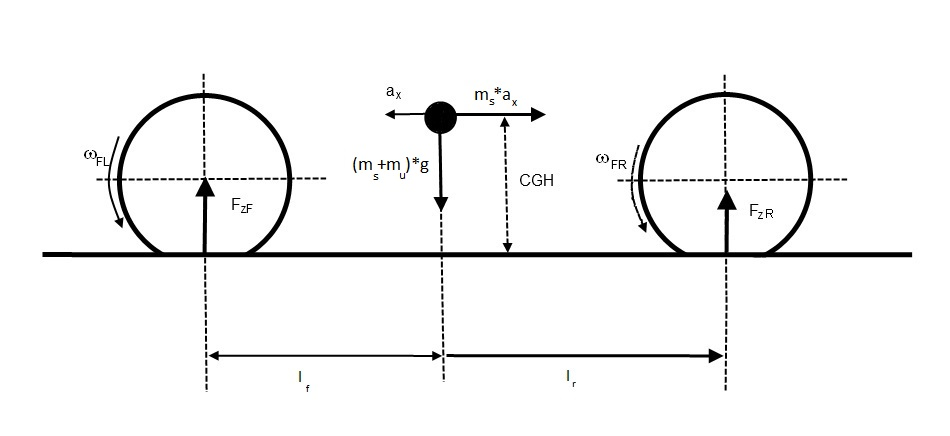
\includegraphics[width=0.8\textwidth]{Pictures/normal_force_longitudinal}
	\caption{Normal force on the car seen from the side.}
	\label{normal_force_longitudinal}
\end{figure}
The normal forces on the front and rear for a vehicle without any acceleration, as seen in Figure \ref{eq:normal_with_long_acc}, is simply the gravitational force acting on the car
\begin{equation} \label{eq:normal_2}
	F_{zF} + F_{zR} = mg
\end{equation}
Note that $ F_{zF} $ denotes the normal force of the rear and not the right hand side like in the previous section. With longitudinal acceleration, the normal forces on the on the front respective the rear will change
\begin{equation} \label{eq:normal_with_long_acc}
	F_{zF}*(a+b) = mg*b - m*a_{x}*CGH
\end{equation}
where $ a $ and $ b $ are the distances from the front and rear axles to the center of gravity. As can be seen in equation \ref{eq:normal_with_long_acc}, he normal force on the front axle will decrease with positive longitudinal acceleration. 

\section{Tire dynamics}
A gas inflated tire that is non loaded will have a radius called unloaded radius. When a tire is loaded, and therefore have a normal force acting on it from the road, it will deform against the road creating a contact area. The contact area is proportional to the load, more load gives larger contact area. The deformation of the tire will lead to a shorter distance between the center of the tire and the road, this is the loaded radius. 

A loaded tires contact area against the road can be divided into two, adhesion area and sliding area (Figure \ref{adh_sliding}). The adhesion area is the part of the contact area that's said to adhere to the road, this means that this part haven't reached the friction limit yet, it can still handle more force without sliding. The sliding area is area that has reached the friction limit and thus has begun sliding. How this area is divided depends on a number of factors but it can basically be divided into two cases, longitudinal forces and lateral forces which will be explained further on.
\begin{figure}[h]
	\centering
	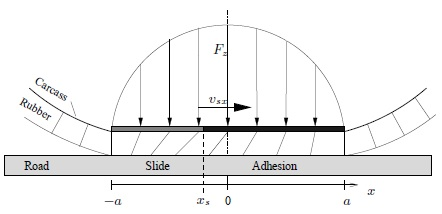
\includegraphics[width=0.8\textwidth]{Pictures/adh_sliding}
	\caption{Adhesion area and sliding area of a tire. \cite{svendenius2013}}
	\label{adh_sliding}
\end{figure}

\subsection{Longitudinal forces}
Rotating the tire will result in compression of the tire where the it hits the road and expansion where it leaves the road. The tire itself has a dampening effect meaning that all energy used to compress the tire won't be recovered when it expands again. This energy loss is called rolling resistance, $ F_{rr} $. $ F_{rr} $ is often modeled as being proportional to $ F_{z} $ with the proportionality constant $ f $ (Equation \ref{eq:rollingres}). A typical value of $ f $ is 0.015 for passenger cars \cite{rajamani}. The compression and expansion of the tire will also move the normal force acting on the tire in front of the center line (Figure \ref{rolling_resistance}) when the tire is rolling. The moved normal force will result in a third radius of the tire, the effective rolling radius. This is the radius related to the actual linear longitudinal velocity of the rolling tire, it's longer than the loaded radius but shorter than the unloaded radius.
\begin{equation}
F_{rr} = fF_{z}
\label{eq:rollingres}
\end{equation}
\begin{figure}[h]
	\centering
	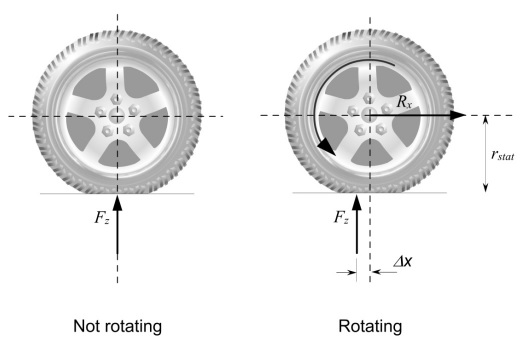
\includegraphics[width=0.8\textwidth]{Pictures/rolling_resistance}
	\caption{Normal force acting on the tire. \cite{rajamani}}
	\label{rolling_resistance}
\end{figure}
Applying torque on the tire will generate longitudinal force moving the tire forwards or backwards. Doing so will always generate a longitudinal slip, called \textit{slip ratio}. This is a ratio of the difference between the angular velocity of the tire and the angular velocity of the corresponding (left or right) undriven wheel. The slip ratio is defined as: 
\begin{equation}
\kappa = \dfrac{R_{e}\omega-V_{x}}{V_{x}}
\label{eq:longslip}
\end{equation}
This leads to the following slip relationships:
\begin{equation}
Locked: \omega = 0 \Rightarrow \kappa = -1
\end{equation}
\begin{equation}
Free rolling: \omega = \frac{V}{R_{e}} \Rightarrow \kappa = 0
\end{equation}
\begin{equation}
Spinning: \omega = 2\frac{V}{R_{e}} \Rightarrow \kappa = 1
\end{equation}
The amount of slip will be one of the factors that decide the ratio between adhesion area and slip area for the tires contact area. The more slip the bigger slip area. The slip area will grow with the slip from the backside of the contact area. When the sliding area is as big as the contact full tire spin occurs. When braking the sliding area will grow from the front and be as big as the contact area when the tire is completely locked. With the same analogy the adhesion area will be as big as the contact area when the tire is free rolling. 

The maximum longitudinal force that can be generated is proportional to the normal force with the friction coefficient as proportionality constant:
\begin{equation}
F_{x} =  \mu F_{z}
\label{eq:fxmufz}
\end{equation}
The friction constant depends on the longitudinal slip, hence the longitudinal force depends on the slip and this is the key to maximizing grip while accelerating or braking.
\begin{figure}[h]
	\centering
	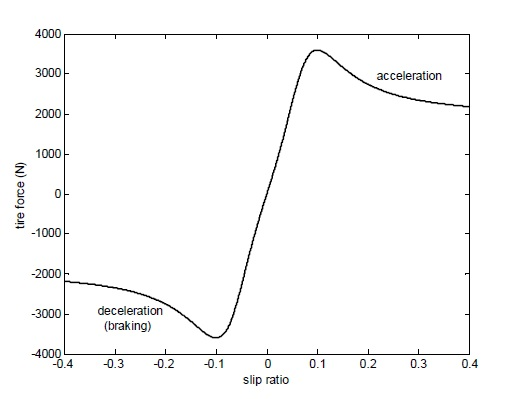
\includegraphics[width=0.8\textwidth]{Pictures/fric_slip}
	\caption{Friction coefficient as a function of slip ratio for a tire. \cite{gustafsson1997}}
	\label{fric_slip}
\end{figure}
As can be seen in Figure \ref{fric_slip} there is a clear maximum of the friction coefficient at a specific slip when driving on good surfaces as asphalt. Hence this is the desired slip when accelerating or braking.

\subsection{Lateral forces}
Lateral forces will be generated when the vehicle is turning, more specifically when there is a difference in the angles of the front tires relative the angle of the vehicle. When turned, the tire won't travel in the direction of its orientation, there will be a slip between the tires orientation and the velocity vector. This lateral slip is called \textit{slip angle} since it can be expressed as an angle.

As can be seen in Figure \ref{slipangle_latforce} the lateral force is proportional to the slip angle for small slip angles. For larger slip angles the lateral force converges. In difference to the longitudinal force the lateral force won't decrease for very large slip. This doesn't mean that max steering wheel angle always generates maximum lateral force. In many situations a too large steering wheel angle will over turn the wheel and start decreasing the slip angle hence generating less lateral force.
\begin{figure}[h]
	\centering
	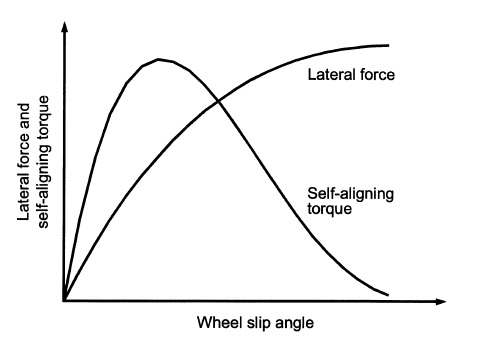
\includegraphics[width=0.8\textwidth]{Pictures/slipangle_latforce}
	\caption{Lateral force as a function of slip angle for a tire. The self aligning torque can also be seen. \cite{sae2004}}
	\label{slipangle_latforce}
\end{figure}

The slip angle is another factor that will decide the ratio between adhesion area and sliding area. When the slip angle is large enough the whole contact area will be in the sliding region, hence the maximum lateral force is generated.

In Figure \ref{slipangle_latforce} the self-aligning torque can also be seen. This is a force generated due to the uneven force distribution over the tires contact area when it's turned. This force increases fast for small slip angles and is the counter force felt in the steering wheel when turning. At a certain point it drops again and this is the locking feeling that's felt in the steering wheel when turning sharp enough.

\subsection{Combined slip}
Since the longitudinal and lateral forces depends on slip ratio and slip angle it's necessary to combine these slips to be able to combine the forces. The total force in any direction can never exceed the normal force times the friction coefficient:
\begin{equation}
F_{total} \leq \mu F_{z}
\label{eq:fmax}
\end{equation}
The total force can be expressed as:
\begin{equation}
F_{total} = \sqrt{F_{x}^{2}+F_{y}^{2}}
\label{eq:ftotal}
\end{equation}
Figure \ref{combined} describes these relations well.
\begin{figure}[h]
	\centering
	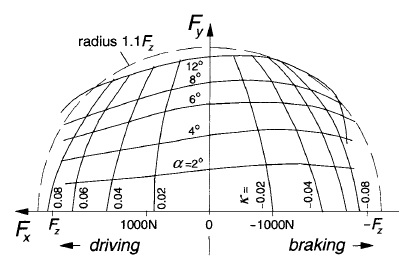
\includegraphics[width=0.8\textwidth]{Pictures/combined}
	\caption{Longitudinal force and slip ratio on the x-axis and lateral force and slip angle on the y-axis. These forces combined can not exceed the circle (Equation \ref{eq:ftotal}) that is the total force expressed as Equation \ref{eq:fmax}. \cite{pacejka}}
	\label{combined}
\end{figure}
It has also been mentioned that both slip ratio and slip angle affects the ratio between adhesion area and sliding area. In analogy with Figure \ref{combined} the sliding areas generated by slip ratio and slip angle will be combined.
\section{Tire models}
There are several models to describe a tire mathematically. These models can be divided into four categories, empirical models, semi-empirical models, simple physical models and complex physical  models. 

Empirical models describe tire characteristics that are acquired from measurements of the tire. To fit the curve according to measured data the parameters are assessed with methods like regression. A well-known empirical model is the Magic Formula \cite{pacejka}. This model provides good fit for $F_{x}$, $F_{y}$ and $M_{z}$ curves and have coefficients that's easy to interpret.

Models using for example the similarity method are semi-empirical which means that some calculations are replaced by known or measured data. By distorting, rescaling and multiplying the result new relationships are acquired which can describe the tire in different situations. For example one can observe that that the pure slip curves shape doesn't change much \cite{pacejka} when the tire runs on different conditions. By shifting the nominal curve these conditions can be described.

The physical models are purely analytical and aims to describe the tire with the help of its physical characteristics. A simple physical model uses simple mechanical representation and can be calculated fairly easy by hand. This often results in pretty poor accuracy but sometimes that's enough. To get better accuracy a more complex model can be set up and simulated in a computer using aids like the finite element method. 

\begin{figure}[h]
	\centering
	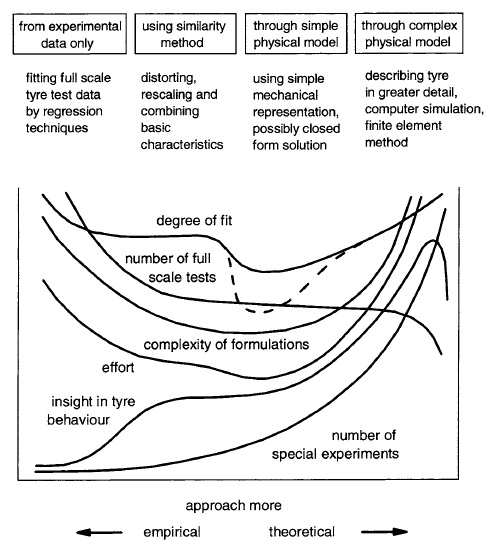
\includegraphics[width=0.8\textwidth]{Pictures/tire_modeling}
	\caption{Four categories of possible types of approach to develop a tire model. \cite{pacejka}}
	\label{tire_modeling}
\end{figure}

In Figure \ref{tire_modeling} some modeling characteristics and how they behave depending on category can be seen.

\subsection{Brush model}
\label{sec:brush}
The \textit{brush model} is a highly used \textit{simple physical model}. The idea is to model the tire surface as a row of elastic bristles that deflects in different directions depending on how the tire is loaded. This model is illustrated to the left in Figure \ref{brush1}.

\begin{figure}[h]
	\centering
	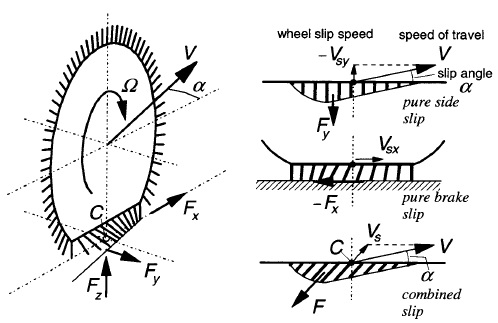
\includegraphics[width=0.8\textwidth]{Pictures/brush1}
	\caption{The brush tire model. \cite{pacejka}}
	\label{brush1}
\end{figure}

For pure side slip the bristles will deflect in the direction of the y-axis, this can be seen at the top right in Figure \ref{brush1}. In the same figure pure brake slip can be seen, that is when the bristles deflects in the direction of the x-axis. Finally at the bottom right of this figure combined slip is illustrated.

\begin{figure}[h]
	\centering
	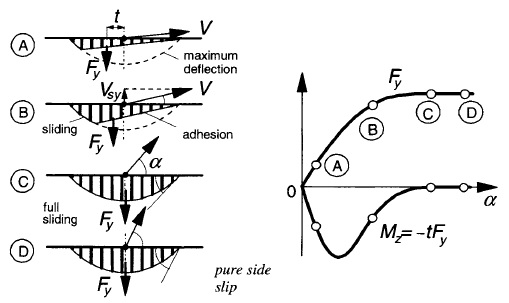
\includegraphics[width=0.8\textwidth]{Pictures/brush2}
	\caption{The brush tire model. \cite{pacejka}}
	\label{brush2}
\end{figure}

In Figure \ref{brush2} it can be seen how different slip angles affects the tire. Small slip angles gives a large adhesion area (flat part) and a small sliding area (curved part). As the slip angle increases a larger number of bristles reaches their maximum deflection, hence increasing the sliding area. At a certain slip angle all bristles have reached their maximum deflection and this results in full sliding. 

\subsection{The Magic Formula Tire Model}

The magic formula is a series of tire design models developed by H. Pacejka \cite{pacejka} in collaboration with Volvo. The formula is a well known empirical model which has been given its name due to no physical basis for the structure of the equation. It models the fact that different tires has various characteristics which influence the final force generated from the contact patch to the ground. The formula is very complex, where these numerous parameters for each tire can be used to calculate lateral and longitudinal forces and also self aligning torque depending on the slip angle or slip ratio. In this report, the magic formula is kept fairly simple to show the idea behind the model, rather than getting a profound understanding behind the development of the model.


\begin{figure}[h]
	\centering
	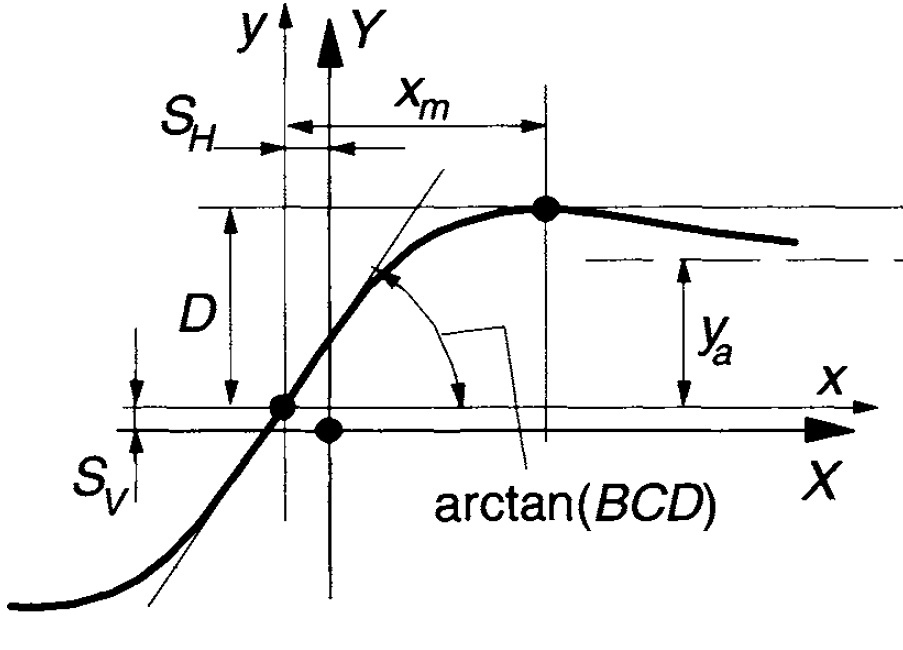
\includegraphics[width=0.8\textwidth]{Pictures/magic_formula}
	\caption{The parameters influence on the magic formula. \cite{pacejka}}
	\label{magic_formula}
\end{figure}

The formula follows
\begin{equation}
	y = Dsin[CarctanBx-E(Bx-arctanBx)]
\end{equation}
where the four fixed constants are

B stiffness factor

C shape factor

D peak factor

E curvature factor

$ y $ is the output, either lateral or longitudinal force, dependent on $ x $ which is the slip angle, $ \alpha $, or slip ratio, $ \kappa $. The input and output can be affected by a offset, $ S_{V} $ and $ S_{H} $, so the curve doesn't pass through the origin.
\begin{equation}
	Y(X) = y(x) + S_{V}
\end{equation}
\begin{equation}
	x = X + S_{H}
\end{equation}
The stiffness factor, $ B $, depends on the cornering stiffness, $ C_{F\alpha} $.
\begin{equation}
	B = \dfrac{C_{F\alpha}}{CD}
\end{equation}
\begin{equation}
	C_{F\alpha} = c_{1}sin(2arctan(\dfrac{F_{z}}{c_{2}}))
\end{equation}
where $ c_{1} $ and $ c_{2} $ is the maximum cornering stiffness respective the load at maximum cornering stiffness.

D is the maximum lateral or longitudinal force
\begin{equation}
	D = \mu F_{z}
\end{equation}
The shape and curvature factors can be described as
\begin{equation}
	C = 1 \pm (1 - \dfrac{2}{\pi}arcsin\dfrac{y_{a}}{D})
\end{equation}
\begin{equation}
	E = \dfrac{Bx_{m} - tan{\dfrac{\pi}{2C}}}{Bx_{m} - arctan(Bx_{m})}
\end{equation}
Where $ x_{m} $ is the distance on x-axis from $ x_{0} $ to the peak of the curve. And $ y_{a} $ is the distance on the y-axis from $ y_{0} $ to the point that the curve converges. Look at Figure \ref{magic_formula} for help.
\subsection{Dugoff tire model}
The longitudinal force described by the Dugoff tire model is defined as:

\begin{equation}
F_{x} = f_{i}*\frac{C_{x} \cdot \kappa}{1-\kappa}
\end{equation}
Where
\begin{equation}
\;\;\;\;\;\;\, f_{i} = \lambda*(2-\lambda) \;\;\;\;\;\;\;\;\; \text{if } \lambda < 1
\end{equation}
\begin{equation}
f_{i} = 1 \;\;\;\;\;\;\;\;\;\;\;\;\;\;\;\;\;\;\;\;\;\;\;\; \text{else}
\end{equation}
\begin{equation}
 \lambda = \mu \cdot F_{z} * \frac{(1-\kappa)}{2 \cdot C_{x} \cdot \kappa}
\end{equation}
The model depends on four parameters; the slip ratio, the longitudinal tire stiffness, the normal force and the tire/road friction coefficient. Assuming that the slip ratio is the only dynamic parameter during driving, means that $ \lambda $ will be smaller than 1 when the slip ratio is small enough. When $ f_{i} = 1 $ the force will only depend on the longitudinal tire stiffness and the slip ratio, meaning that the friction coefficient and normal force has no impact. 

\subsection{Tire model by Ola}

Three different regions. Three parameters describing the curve: max force slip (at $ \mu = 1$), curvation $ Xsi $ and slope at zero slip $ C_{x} $.

\section{Differentials}
When driving in a straight line on a road with equal friction for all wheels, both driven wheels will have equal torque and velocity. In this situation a differential wouldn't even be necessary. The differential is needed when the vehicle is cornering. In this situation the different wheels will have different turning radii, thus requiring different angular velocities. This is the general idea behind a differential, to be able to have different angular velocities of the driven wheels. Without a differential it would be very hard to turn the vehicle, especially at low speeds, since equal speed of the wheels prevents the rotating movement happening while turning.

\subsection{Open differential}
The open differential is the classic differential used in most cars today. With an open differential, the torque will always be evenly distributed to the two driving wheels. One wheel can not have higher torque than the other wheel but they can have different angular velocities. This behavior is directly related to the mechanical construction of the open differential which can be seen in Figure \ref{wikidiff}. 
\begin{figure}[h]
	\centering
	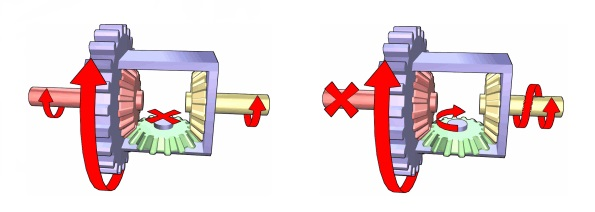
\includegraphics[width=0.8\textwidth]{Pictures/opendiff}
	\caption{The open differential. To the left the case of equal wheel speed, to the right is one wheel completely stationary while the other wheel still rotates. \cite{wikidiff}}
	\label{wikidiff}
\end{figure}
The angular velocities of the two side gears and the crown wheel can be described as:
\begin{equation}
\omega_{r} = \frac{\omega_{1} + \omega_{2}}{2}
\label{eq:diff}
\end{equation}

\subsection{Problems with the open differential}
A situation that creates a problem for a vehicle with an open differential, is when one driven wheel has significant lower friction to the ground than the other. The wheel with low friction can only handle relatively low torque before it starts spinning. This means that the torque applied to the two drive shafts will be restricted by the wheel with the lowest friction to the ground due to the torque splitting nature of the open differential. This will in turn reduce the traction of the car. Two possible scenarios for when the friction to the ground might differ between the driven wheels are when the road is partly covered in ice and when cornering at high speeds which will make the inner wheel lift from the ground. 

When driving on a split-$ \mu $ (different friction coefficients for the driven wheels) surface, the wheel on the low friction area will easily reach maximum force before it starts to spin. The force it can transfer to the ground will thus be the restricted which in turn will restrict the torque applied on the other wheel. The result of all this is that even though only one wheel has bad grip to the ground the traction is still greatly reduced.

The other scenario, when cornering at a high speed leading to the inner wheel lifting, will give the same effect. The normal force acting on the inner wheel will be reduced when it lifts. This will reduce the force that can be transfered to the ground which will reduce the amount of torque that can be applied to the drive shafts. In a worst case scenario the inner wheel has lost contact to the ground completely reducing the transfered force to the ground to zero. The only torque applied is to spin the wheel and this is almost no torque at all compared to the torque used to propel the the car. The propulsive power will be zero and the car will lose speed. After a while the inner wheel will touch the ground again and some force will be transfered only to lift the wheel up again. This will get the car stuck oscillating around this inefficient boundary wasting lots of power.

A solution for these two different scenarios would be to lock the two drive shafts together. This would keep torque applied to the outer wheel even when the inner wheel loses grip, but the fundamental idea of the differential would be lost. That is, the possibility of a speed difference between the two drive shafts. This would also affect the steering behavior in several bad ways, especially at lower speeds. Hence it would be very beneficial to be able to lock the drive shafts together in certain situations. It would be even more beneficial if they were coupled with a device where some slip were allowed between the shafts, making it possible to control the amount of torque transfered from one shaft to the other. Enter, the limited slip differential.

\subsection{Limited slip differential}
The idea of a limited slip differential (LSD) is not to apply more torque to a wheel than it can transfer to the ground. This means that the torque splitting nature of an open differential needs to be countered. Take the sharp turn example from above. The lateral forces of the car will lift the inner wheel from the ground which will result in less traction. With a LSD the torque distribution can be managed so that more torque is applied on the outer wheel. The car will gain more traction when cornering with a LSD than with an open differential. The same effect is applied when driving on a split-$ \mu $ surface. Torque is transfered from the wheel with lower friction to the ground to the wheel with higher friction to the ground to increase the traction.

There are different types of LSDs, they can be divided in two main categories, passive and active LSDs. Passive LSDs are designed in such a way that they do the torque distribution without any required activity from the outside. The Torsen differential is a brilliant example of a passive differential. A complex set of worm gears and spur gears results in a differential that does the torque distribution by itself when needed. Passive differentials require little effort to use but the properties of the differential can't be changed in any way.

Active differentials are controlled from the outside. The amount of torque transfered from one shaft to the other can be freely controlled and this gives much more power over the cars behavior.

\subsection{FXD}
The FXD is an active limited slip differential made by BorgWarner AB for FWD cars. It uses the same clutch technology as their four wheel drive systems. Instead of using the clutch to transfer torque between front and rear it's used to transfer torque between the left and right front wheels. The fact that the clutch is actuated from the outside is what makes the FXD an active limited slip differential, the torque transfered between the wheels is freely controlled.

\subsubsection{The clutch}
The clutch is based on BorgWarner's Gen5 clutch. This is an electro-hydraulic basket clutch. The clutch is engaged by building a hydraulic pressure in the clutch forcing the clutch plates together resulting in a torque transfer. The pressure is built up by a hydraulic pump operated by an electric DC motor. A the quick and exact control nature of the DC motor results in the clutch being very accurate. The amount of torque transfered through the clutch is easily managed with a rather simple electric signal and above all changed can be made very quick. This is positive when used in cars because things happens very fast.

\subsubsection{The differential}
The differential is basically an open differential but with one major difference, the electro-hydraulic clutch. The clutch is installed in a way that makes it possible to couple one of the drive shafts together with the differential housing. This gives the possibility to transfer torque from one shaft to the other in certain situations. One of these situations is when one wheel has less grip than the other wheel, torque can then be transfered to the wheel with the most grip. When cornering hard or driving on a split-$ \mu $ surface the clutch will be engaged allowing for the torque distribution to be altered.

\subsubsection{Control algorithm}
It's been stated that the FXD itself is very easy to control but to get any real function from it needs to be controlled in a smart way. The algorithm controlling the FXD is complex and powerful. It uses several measured signals from the car which it receives via the CAN bus to calculate the best possible amount of torque to transfer at any time while driving. 

\subsubsection{Benefits of the FXD}
The most obvious benefit of being able to distribute torque freely between the driven wheels is used in several ways to create even more benefits. The overall traction of the car when cornering or running on split-$ \mu $ surface is improved to begin with. Since it's an active LSD it's much easier to avoid heavy under steer compared to passive LSDs where the locking torque can't be controlled at any given moment. It's a lightweight alternative compared to AWD to improve traction performance and it can prevent torque steer.

A major safety benefit is the yaw damping feature. Being able to lock the driven wheels together in an avoidance maneuver will make the car less likely to spin out of control since the locked wheels will prevent the car from rotating around its own axle. Another benefit to safety is the fact that it's an active LSD. This means that torque transfer can cease immediately in favor of the ABS and ESP systems when needed. When this need to happen really fast the DC motor operating the hydraulic pump is short circuited which will make it stop instantaneously releasing all pressure on the clutch. 